%%%%%%%%%%%%%%%%%%%%%%%%%%%%%%%%%%%%%%%%%%%%%%%%%%%%%%%%%%%%%%%%%%%%%%%
% How to use writeLaTeX: 
%
% You edit the source code here on the left, and the preview on the
% right shows you the result within a few seconds.
%
% Bookmark this page and share the URL with your co-authors. They can
% edit at the same time!
%
% You can upload figures, bibliographies, custom classes and
% styles using the files menu.
%
%%%%%%%%%%%%%%%%%%%%%%%%%%%%%%%%%%%%%%%%%%%%%%%%%%%%%%%%%%%%%%%%%%%%%%
\documentclass[a4paper]{article}

%\usepackage{orcidlink}

\usepackage{renote-template}
\usepackage{graphicx,url}
\usepackage[brazil]{babel}
\usepackage[utf8]{inputenc}  
\usepackage{longtable}
\usepackage[none]{hyphenat}
\usepackage{fancyhdr}
\usepackage{setspace}
%\usepackage{hyperref}



\usepackage[dvipsnames]{xcolor}
\usepackage[alf, bibjustif, abnt-etal-list=5, abnt-emphasize=bf,
            abnt-etal-text=it, abnt-repeated-author-omit=no        ]{abntex2cite}

\fancyhf{}
\fancyhead[C]{\thepage}
\pagestyle{fancy}
\sloppy
\singlespacing


\title{Análise da evasão feminina nos cursos de Ciência da Computação das universidades públicas e presenciais de Santa Catarina}


\author{
\fontsize{10pt}{10pt}\selectfont
    Maria Teresa Silva Santos, UDESC, maria.santos2805@edu.udesc.br, 0000-0001-8093-2446
    \\
    \fontsize{10pt}{10pt}\selectfont
    Laís Pisetta Van Vossen, UDESC, lais.vossen@edu.udesc.br, 0000-0002-1725-0618
    \\
    \fontsize{10pt}{10pt}\selectfont
    Daniella Vasconcellos, UDESC, daniella.vasconcellos@edu.udesc.br, 0000-0001-9250-8116
    \\
    \fontsize{10pt}{10pt}\selectfont
    Guilherme Tomaselli Borchardt, UDESC, guilherme.borchardt@edu.udesc.br, 0000-0002-7809-0590 
    \\
    \fontsize{10pt}{10pt}\selectfont
    Gabriel Vaichulonis, UDESC, 	gabriel.vaichulonis@edu.udesc.br, 0000-0003-3676-7441
   \\
   \fontsize{10pt}{10pt}\selectfont
   Luciana Bolan Frigo, UFSC, luciana.frigo@ufsc.br, 0000-0002-0156-2959
   \\
  \fontsize{10pt}{10pt}\selectfont
   Isabela Gasparini, UDESC, isabela.gasparini@udesc.br, 0000-0002-8094-9261
   \\
}

\begin{document} 

\maketitle

\begin{resumo} 

De acordo com o Instituto Nacional de Estudos e Pesquisas Educacionais Anísio Teixeira (INEP) as mulheres são maioria no ensino superior brasileiro, no entanto no escopo dos cursos de computação essa realidade é muito diferente. Tendo isso em vista, apresenta-se aqui uma análise dos dados públicos do ensino superior brasileiro, com foco nos cursos de bacharelado em Ciência da Computação nas universidades de ensino presencial e públicas do estado de Santa Catarina, abrangendo os anos de 2015 a 2019. O trabalho tem como objetivo apresentar as relações comparativas entre gênero, evasão e demais fatores impactantes como raça, forma de ingresso e idade. Como resultado, apresenta-se uma grande disparidade no número de homens e mulheres nos cursos analisados, observando a maior evasão em ambos os gêneros acima de 35 anos.
\end{resumo}

\begin{palavas-chave}
    Mulheres, Ensino superior, Evasão, Ciência da Computação, Análise de dados.
\end{palavas-chave}

\begin{englishtitle}
    Analysis of female student dropout within Computer Science courses at public and in-class universities in Santa Catarina
\end{englishtitle}

\begin{abstract}
%ARRUMAR INGLÊS
Accordingly to Instituto Nacional de Estudos e Pesquisas Educacionais Anísio Teixeira (INEP) women are the majority in Brazilian higher education, however in the scope of computing courses this reality is very different. In view of this, we present here an analysis of the public data of Brazilian higher education, focusing on the bachelor's degrees in computer science in public and presential universities in the state of Santa Catarina, covering the years 2015 to 2019. The study aims to present the comparative relationships between gender, evasion and other impacting factors such as race, form of entry and age. As a result, there is a great disparity in the number of men and women in the analyzed courses, with the highest dropout rate in both genders over 35 years old.
\end{abstract}

\begin{keywords}
    Women, Higher Education, Dropout, Computer Science, Data analysis.
\end{keywords}


\section{Introdução}
\renewcommand{\thefootnote}{\arabic{footnote}}
Análises de dados educacionais possuem grande relevância em diversos contextos. No Brasil tais dados são fornecidas pelo Instituto Nacional de Estudos e Pesquisas Educacionais Anísio Teixeira (INEP\footnote{https://www.gov.br/inep/pt-br/acesso-a-informacao/dados-abertos/microdados}), sendo utilizados para diversos estudos e análises com o intuito de compreender melhor os aspectos sobre a educação brasileira, além de ser possível realizar predições de estudantes que podem evadir, e contribuindo no desenvolvimento de políticas públicas para a retenção desses estudantes.

Outro fator importante da análise de dados é a possibilidade de observar as disparidades de gênero presentes na educação. Embora a participação da mulher na educação superior de maneira geral seja expressiva, como mostrado por \citeonline{suzane:2018} ao concluírem que as mulheres possuem 53,8\% das matrículas nas universidades públicas e 58,6\% nas particulares, esse cenário não é igualitário em todas as áreas da ciência. A mulher tem uma menor representatividade nos cursos de tecnologia, como mostra \citeonline{marcel:2016} o qual explicitou que entre 2000 e 2013, apenas 17\% dos concluintes eram do gênero feminino. Esse fenômeno se replica não apenas no Brasil, mas também em universidades de outros países, como os Estados Unidos \cite{lunn:2021}. De acordo com \citeonline{NCWIT:2020}, em meados dos anos 80, 40\% dos diplomas em Ciência da Computação nos Estados Unidos eram de mulheres, ao passo que em 2013, elas representaram somente 18\% dos estudantes graduados, e ainda, que o curso de Ciência da Computação seja o único curso onde a disparidade de gênero tenha tido um aumento nas últimas décadas.

Considerando este cenário apresentado, o objetivo deste trabalho é obter um panorama do cenário acadêmico dos cursos de Ciência da Computação do estado de Santa Catarina, em instituições classificadas de acordo com o MEC, através da plataforma do e-MEC\footnote{https://emec.mec.gov.br/}, como públicas, presenciais e com grau de bacharelado, com enfoque nas relações entre gênero e a evasão escolar. Para tal, são feitas análises estatísticas dos dados de evasão coletados do INEP. %São observadas diferenças na evasão entre homens e mulheres captando outras características que influenciam na mesma. %<- Isso é resultado e não deve aparecer na Introdução 

Para tanto, pretende-se responder às seguintes questões de pesquisa definidas neste trabalho: \textbf{Q1:} Qual a diferença entre estudantes homens e mulheres para cada instituição de ensino e ano analisados? \textbf{Q2:} Como se apresentam as taxas de evasão separadas por gênero nessas mesmas instituições e anos? \textbf{Q3:} Qual a relação entre faixa etária e gênero com a taxa de evasão? \textbf{Q4:} Qual a relação entre forma de ingresso no ensino superior e gênero com a taxa de evasão? \textbf{Q5:} Qual a relação entre raça e gênero com a taxa de evasão? O presente artigo está dividido em seis seções. A seção 2 apresenta o conceito de evasão e os trabalhos relacionados. A seção 3 discute os procedimentos metodológicos. A seção 4 apresenta a análise dos dados observados. Na seção 5 a discussão dos resultados e por fim na seção 6 as considerações finais do trabalho. 

% \textcolor{red}{Tamanho da folha: para  impressão em papel  A4 (21,0 cm x 29,7 cm) sendo observadas as seguintes margens: superior 3,0; cm inferior 2,0 cm; esquerda e direita 3,0 cm. Alinhar a margem direita evitando separações silábicas com barras ou outros sinais. Utilizar fonte "Times" tamanho 12 ou equivalente. Não utilizar fontes que ocupam muito espaço tal como "Bookman".  No texto utilizar espaço 1.  O fim de uma seção e o cabeçalho da próxima são separados por um espaço extra.  Todas as páginas do trabalho devem ser numeradas, com exceção da folha de rosto.  Os números, em algarismos arábicos, são colocados, no centro da margem superior. Sugere-se utilizar o comando "cabeçalho" do editor de texto para especificar a paginação. Entre a paginação e o texto deixar algum espaço para destacar os dois elementos. }

\section{Evasão Escolar} 
Entender a evasão é um processo necessário para a busca por sua solução, que mostra-se complexa e cada vez mais próxima do campo da computação, na tentativa de desvendá-la. Diferentes conceitos são encontrados na literatura, para \citeonline{utiyama:2003} a evasão é um conceito mais amplo, não estabelecendo nenhum critério de tempo para saída do estudante de seu curso, entendendo assim como evasão a saída definitiva de seu curso, a não conclusão. Já \citeonline{abbad:2005} conceitua evasão como desistência definitiva do estudante em qualquer etapa do curso, não deixando claro se inclui nesse conceito os estudantes que se matricularam e não iniciaram o curso. \citeonline{maia:2005} consideram os estudantes evadidos os que não completaram o curso ou programa de estudo, e também aqueles que se matriculam e desistem antes mesmo de iniciar o curso.

Por existir uma série de classificações, \citeonline{stratton:2008} e \citeonline{montmarquette:2001} sugerem três tipos de evasão, abandono definitivo do curso (\textit{Dropout}), mudança de curso ou instituição (\textit{Optout}) e pausa por um período de tempo (\textit{Stopout}). Tendo em vista que a evasão pode ser conceituada de diversas maneiras, é importante ressaltar que para o presente artigo adota a definição do \citeonline{dados:2017}, que considera a evasão como a ``saída antecipada, antes da conclusão do ano, série ou ciclo, por desistência (independentemente do motivo)''. Vale ressaltar que não é entendido como evasão apenas o caso de interrupção devido ao óbito do discente, pois em tal situação não é possível presumir que houve uma intenção, vinda do estudante, de interromper sua formação.




%\subsection{Trabalhos Relacionados}\label{Trabalhos Relacionados}

Alguns trabalhos relacionam-se com o presente artigo, analisando o cenário feminino no meio da computação e nos cursos de exatas. Segundo \citeonline{moreira:2018} em 2015 as mulheres representaram 55,6\% das matrículas em andamento em cursos superiores no Brasil e 59,9\% das concluintes. Mas essa realidade não se reflete para todas as áreas do conhecimento, pois ao se analisar o número de matrículas por  curso, pode-se ver que na área da tecnologia sua presença é muito baixa. Em 2017 na Universidade Federal de Paraíba, das matrículas ativas em Ciência da Computação, Engenharia de Computação e Matemática Computacional, as mulheres representavam 10,2\%, 13,8\% e 21\%, respectivamente.
    
Além disso, é possível observar o cenário da Universidade de Brasília que oferece 3 cursos de pós-graduação em Ciência da Computação, mestrado acadêmico, mestrado profissional e doutorado acadêmico, desde 2006 até 2019 foram defendidas 280 dissertações e teses sendo que destas, 21 foram de teses, 163 defesas de dissertações do mestrado acadêmico e 103 defesas de dissertações no mestrado profissional. Das teses defendidas, 3 foram de mulheres, das dissertações do mestrado acadêmico, apenas 25, e das dissertações no mestrado profissional, 12 \cite{holanda:2019}.
    
No cenário das exatas, de acordo com \citeonline{sigolo:2021} em 2017 o Censo de Educação Superior do INEP viu que no Brasil, 29,3\% dos estudantes de cursos de engenharia eram mulheres. Enquanto isso, nos cursos de Ciência da Computação a mulher tinha uma presença de 15\% de estudantes. Ademais, segundo a Pesquisa Nacional por Amostra de Domicílio realizada em 2016 pelo Instituto Brasileiro de Geografia e Estatística, as mulheres que trabalham nas áreas de Tecnologia da Informação representam apenas 20\% dos profissionais que atuam no país.

\section{Procedimentos Metodológicos}\label{ProcedimentosMetodologicos}

O presente artigo considera o curso de Ciência da Computação das Instituições de Ensino Superior (IES) públicas do estado de Santa Catarina como cenário de pesquisa. A escolha deste cenário se deu por Ciência da Computação fazer parte dos cursos da área de STEM, sigla em inglês para \textit{Science, Technology, Engineering and Mathematics} (Ciência, Tecnologia, Engenharia e Matemática, em português), que em uma tendência mundial apresenta um número baixo de mulheres. Já a escolha do estado de Santa Catarina se deu por ter sua capital como um polo tecnológico de referência, além de ser o estado que mais cresceu em número de empresas de tecnologia em 2020 \cite{digital_2020}. %\cite{willerding:2017}

No cenário Brasileiro, é possível observar de acordo com \citeonline{unesco:2018} que a participação de mulheres deve ser considerada no contexto de seu acesso e envolvimento em todos os níveis educacionais, alinhando-se também com a Agenda 2030 para o Desenvolvimento Sustentável, nos objetivos 4 e 5, que respectivamente falam sobre a educação inclusiva, equidade da qualidade e aprendizagem ao longo da vida e sobre a igualdade de gênero e empoderamento das meninas e mulheres.

%\citeonline{unesco:2018} Brasil \citeyear{unesco:2018}
O relatório produzido pela \citeonline{unesco:2018} ressalta questões importantes e apresenta especialmente que abordar questões de gênero na área de STEM traz novos caminhos e abre portas tanto para meninos e homens, quanto para meninas e mulheres, fazendo os seres humanos mais capazes de construírem novas habilidades, trazendo então diversas oportunidades, benefícios igualitários e todas as vantagens associados a esta área.

As análises apresentadas na seção \ref{analisedosdados} foram feitas a partir de dados fornecidos pelo INEP. Todas as análises apresentadas baseiam-se na divisão de gênero disponível no banco de dados, as variáveis mostradas são apenas feminino e masculino, bem como todas as outras divisões de cor e raça e forma de ingresso.

Com relação às classificações binárias de gênero, sabe-se que é uma construção cultural, social e historicamente trata-se de um vetor capaz de identificar aspectos e relações de poder entre homens e mulheres, influenciando inclusive na decisão de qual curso deve-se ou não frequentar \citeonline{uamusse:2020}. Vale salientar a importância de uma classificação de gênero mais diversa e que retrate a realidade, tendo em vista a pluralidade no mundo que nos cerca.

Quanto ao tratamento e a análise dos dados, utilizam-se os microdados do censo da educação superior disponibilizados pelo INEP, disponíveis desde 1995. Neste artigo, o período estudado foi de 2014 a 2019. Foram utilizados os arquivos referentes aos cursos superiores, aos estudantes e às instituições de ensino. Para todos os anos os arquivos foram disponibilizados em formato CSV. Para facilitar a compreensão dos dados, junto ao banco de informações, em cada censo da educação superior, um dicionário de variáveis é disponibilizado pelo INEP. Quanto a limpeza e preparação dos dados, foi utilizada a linguagem de programação \textit{Python} para fazer o recorte ano a ano, já que os arquivos CSV individuais possuem aproximadamente 4 Gigabytes, o que dificulta na leitura e processamento do arquivo sem a limpeza.
 
\\
\section{Análise dos dados}\label{analisedosdados}
A partir de todos os dados disponíveis, além de toda a limpeza dos dados, foram realizados alguns recortes, selecionando apenas as instituições de ensino do estado de Santa Catarina que possuem o curso de Ciência da Computação, classificadas como públicas, presenciais e com grau de bacharelado. Tais recortes emergiram dos filtros de busca disponíveis no Cadastro Nacional de Cursos e Instituições de Educação Superior, disponíveis no e-MEC. As análises presentes no decorrer do artigo são referentes aos dados dos Censos de 2015 até 2019. No período em que as análises foram feitas, até o mês de fevereiro de 2022, a base mais recente disponível era a do ano de 2019. Já o Censo do ano de 2020 foi publicado posteriormente a esta data, desta forma trazemos as análises dos anos seguintes como trabalhos futuros.

Como resultado, 8 Instituições de Ensino foram encontradas, porém o Instituto Federal Catarinense do Blumenau (IFC Blumenau) não retornou nenhum dado, então foi desconsiderado para a presente análise. Desta forma foram selecionadas 7 instituições, que são elas: Universidade Federal de Santa Catarina (UFSC), Universidade Federal da Fronteira Sul (UFFS), Universidade Regional de Blumenau (FURB), Universidade do Estado de Santa Catarina (UDESC), Instituto Federal Catarinense  do Rio do Sul (IFC Rio do Sul),  do Rio do Sul de Videira (IFC Videira) e Instituto Federal de Santa Catarina (IFSC). Vale ressaltar que, embora a FURB não seja uma universidade gratuita, ela é uma autarquia municipal de regime especial e portanto é considerada uma universidade pública, de acordo com os dados do INEP \footnote{https://www.furb.br/web/1317/institucional/a-furb/nossa-historia}.

%, com sede e foro no Município de Blumenau, possuindo todas as prerrogativas e os privilégios da fazenda pública municipal 

% Além das análises gerais e de números absolutos, para a realização das análises sobre as taxas anuais de evasão, os autores estudaram o dicionário de variáveis pertencente a base de dados do Censo da Educação Superior do INEP, durante o processo, foi possível observar outras aplicações que coincidiram com as análises conceituais do que representa a evasão escolar dentro dos dados, como no artigo de \citeonline{silva:2007}, em que os autores calcularam a evasão da seguinte maneira:

% \begin{equation}\label{eq:evasaovelha}
% E(n) = 1– \frac{M(n)–I(n)}{M(n-1)–C(n-1)}
% \end{equation}

% Sendo que \textit{E} é a evasão a ser calculada, \textit{M} é a quantidade de matriculados, \textit{I} é a quantidade de ingressantes, \textit{C} é a quantidade de concluintes, \textit{n} é o ano de referência e \textit{n} - 1 é o ano anterior. \citeonline{silva:2007} analisam os dados dos anos anteriores a 2009, ano em que ocorreu uma mudança na organização dos dados do INEP, sendo assim, a Equação \ref{eq:evasaovelha} aplicada nessa situação não pôde ser utilizada para os anos explorados no presente artigo. 

No ano de 2017, a Diretoria de Estatísticas Educacionais publicou a Metodologia de Cálculo
dos Indicadores de Fluxo da Educação Superior \citeonline{dados:2017}, onde apresentou uma  forma de calcular a Taxa de Desistência Anual (Tada), apresentada na Equação \ref{eq:evasaonova}, e que leva em consideração a nova organização dos dados disponíveis. É importante salientar que a definição adotada de desistência é a mesma da evasão, sendo utilizados como sinônimos ao longo do documento \cite{dados:2017}.

\begin{equation}\label{eq:evasaonova}
{Tada_{j,T,t}} = \frac{\sum_{i=1}^{n_{j,t}} Des_{i,j,t} + \sum_{i=1}^{n_{j,t}} Transf_{i,j,t}} {\sum_{i=1}^{n} IG^T_{i,j} - \sum_{w=T}^{t} \sum_{i=1}^{n_{j,w}} Fal_{i,j,t}} \times{100}
\end{equation}

Para encontrar a porcentagem de evasão em determinado período de tempo, assume-se na Equação \ref{eq:evasaonova} que a variável \textit{j} representa a Instituição de Ensino Superior, \textit{t} é o ano de referência, \textit{T} é o ano de ingresso, nota-se que \textit{t} $\geq$ \textit{T}, \textit{Des} representa o estudante com situação de vínculo igual a “Desvinculado do Curso” no curso \textit{j} no ano \textit{t}, \textit{Transf} os estudante com situação de vínculo igual a “Transferido para outro curso da mesma IES” no curso \textit{j} no ano \textit{t}, \textit{IG} o número total de ingressantes no curso \textit{j} no ano \textit{T} e \textit{Fal} estudante com situação de vínculo igual a “Falecido” no curso \textit{j} no ano \textit{t} e no ano \textit{T}. Nesse contexto é importante ressaltar que o número total de ingressantes (\textit{IG}) não é representado no banco de dados por uma única variável, e sim pela somatória de diversas variáveis, sendo elas o somatório de: Estudantes com situação de vínculo igual a ``Cursando'', ``Matrícula trancada'', ``Desvinculado do curso'', ``Transferido para outro curso da mesma IES'', ``Formado” e  ``Falecido'' no curso \textit{j} no ano \textit{t} mais os Estudantes com situação de vínculo igual a ``Desvinculado do curso'', ``Transferido para outro curso da mesma IES'', ``Formado'' e  ``Falecido'' no curso \textit{j} no ano \textit{T}.

Nas próximas subseções são realizadas análises sobre a taxa de evasão e outros aspectos pertinentes, utilizando a Equação \ref{eq:evasaonova} como base para os cálculos. Com isso, pretende-se apresentar os dados e correlações entre fatores significantes para o contexto da análise de evasão e gênero, porém não tem-se por objetivo debater a causalidade ou os motivos por trás dos resultados obtidos, visto que essa seria uma discussão demasiadamente complexa para ser abordada.
\subsection{Número de mulheres, homens e geral}\label{sec:mulheresehomensgeral}

Na Tabela \ref{tab:my-table}, é possível visualizar as quantidades de homens e mulheres nos cursos de Ciência da Computação das instituições de ensino superior públicas e presenciais do estado de Santa Catarina, e, com os dados apresentados, é clara a percepção da diferença quantitativa entre os gêneros no curso, assim ajudando a explicar a baixa quantidade da presença feminina nos meios profissionais e científicos relacionadas a área.

Observando os dados apresentados na Figura \ref{fig:MulheresHomens}, percebe-se que a UFFS, entre todas as instituições de ensino superior analisadas, é a que possui as maiores quantidades de mulheres no curso durante os cinco anos, chegando a conter 67 alunas no ano de 2019, sendo este o maior número de mulheres presente no gráfico.

\begin{figure}[ht]
\centering
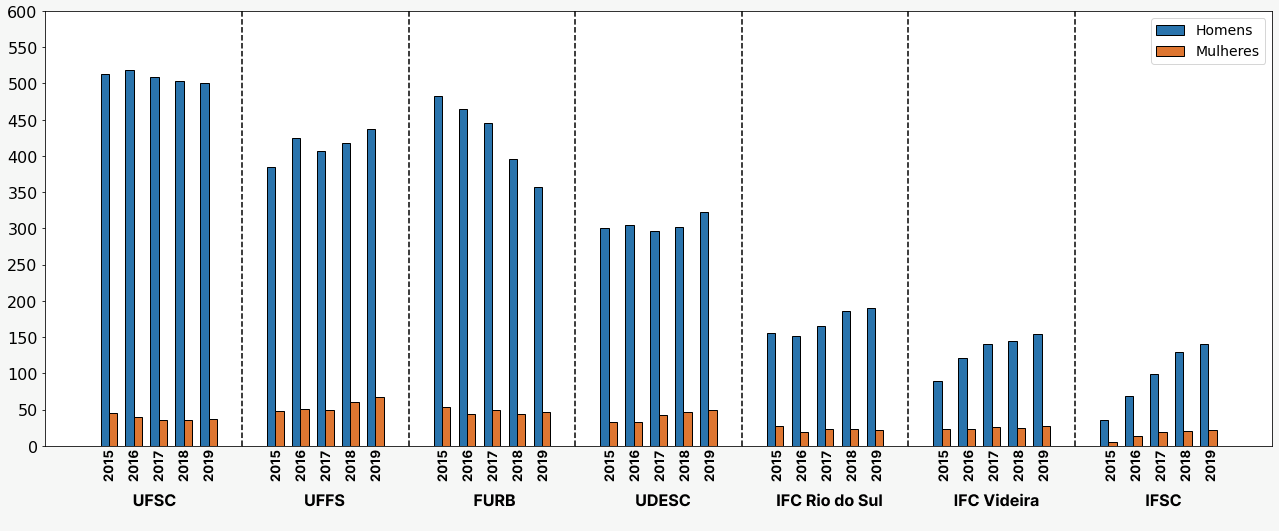
\includegraphics[width=1\textwidth]{Grafico.png}
\caption{Quantidade de estudantes por gênero e Instituição de Ensino Superior}
\label{fig:MulheresHomens}
\end{figure}

Com os dados da Tabela \ref{tab:my-table} é possível observar a partir das porcentagens relativas da presença feminina, que o IFC Videira teve aproximadamente 20,54\% de mulheres no ano de 2015, sendo a com maior representatividade em comparação a todos os anos analisados. Já a UFSC apresenta a menor porcentagem geral, com 6,49\% no ano de 2019.
Fazendo essa mesma análise ano a ano, iniciando em 2015 e indo até 2019, a instituição de ensino com maior porcentagem feminina segue sendo o IFC Videira, com exceção do ano de 2017, em que o IFSC assume essa posição. Na mesma análise, agora observando as instituições com menor presença relativa de mulheres ano a ano, é possível observar que em todos os anos a UFSC continua sendo a com menor presença relativa feminina, sendo que em 2015 apresentou sua maior porcentagem.

Ainda em relação a Tabela \ref{tab:my-table}, observa-se que as médias masculinas em todos os anos se mantêm acima de 87\%. A maior média ocorreu em 2016, onde 88,78\% dos estudantes das instituições analisadas eram homens, enquanto que a maior média feminina foi 12,34\% em 2015. Compreende-se que os cálculos das médias correspondem ao cenário Catarinense dos cursos das instituições de ensino superior públicas e presenciais de Ciência da Computação anualmente.
\begin{table}[ht]
\centering
\caption{Porcentagem de Estudantes Homens e Mulheres Matriculados por Ano e Instituição}
\label{tab:my-table}
\resizebox{\textwidth}{!}{
\begin{tabular}{|c|cc|cc|cc|cc|cc|}
\hline
\multicolumn{1}{|l|}{\multirow{}{}{}} & \multicolumn{2}{c|}{2015}              & \multicolumn{2}{c|}{2016}              & \multicolumn{2}{c|}{2017}              & \multicolumn{2}{c|}{2018}              & \multicolumn{2}{c|}{2019}              \\ \cline{2-11} 
\multicolumn{1}{|l|}{}                  & \multicolumn{1}{c|}{Homem}   & Mulher  & \multicolumn{1}{c|}{Homem}   & Mulher  & \multicolumn{1}{c|}{Homem}   & Mulher  & \multicolumn{1}{c|}{Homem}   & Mulher  & \multicolumn{1}{c|}{Homem}   & Mulher  \\ \hline
UFSC                                    & \multicolumn{1}{c|}{91,94\%} & 8,06\%  & \multicolumn{1}{c|}{92,84\%} & 7,16\%  & \multicolumn{1}{c|}{93,39\%} & 6,61\%  & \multicolumn{1}{c|}{93,51\%} & 6,49\%  & \multicolumn{1}{c|}{93,12\%} & 6,88\%  \\ \hline
UFFS                                    & \multicolumn{1}{c|}{88,91\%} & 11,09\% & \multicolumn{1}{c|}{89,26\%} & 10,74\% & \multicolumn{1}{c|}{89,06\%} & 10,94\% & \multicolumn{1}{c|}{87,27\%} & 12,73\% & \multicolumn{1}{c|}{86,71\%} & 13,29\% \\ \hline
FURB                                    & \multicolumn{1}{c|}{90,11\%} & 9,89\%  & \multicolumn{1}{c|}{91,34\%} & 8,66\%  & \multicolumn{1}{c|}{89,92\%} & 10,08\% & \multicolumn{1}{c|}{90,00\%} & 10,00\% & \multicolumn{1}{c|}{88,37\%} & 11,63\% \\ \hline
UDESC                                   & \multicolumn{1}{c|}{90,12\%} & 9,88\%  & \multicolumn{1}{c|}{90,24\%} & 9,76\%  & \multicolumn{1}{c|}{87,32\%} & 12,68\% & \multicolumn{1}{c|}{86,78\%} & 13,22\% & \multicolumn{1}{c|}{86,79\%} & 13,21\% \\ \hline
IFC Rio do Sul                          & \multicolumn{1}{c|}{85,25\%} & 14,75\% & \multicolumn{1}{c|}{88,89\%} & 11,11\% & \multicolumn{1}{c|}{87,77\%} & 12,23\% & \multicolumn{1}{c|}{89,00\%} & 11,00\% & \multicolumn{1}{c|}{89,62\%} & 10,38\% \\ \hline
IFC Videira                             & \multicolumn{1}{c|}{79,46\%} & 20,54\% & \multicolumn{1}{c|}{84,03\%} & 15,97\% & \multicolumn{1}{c|}{84,34\%} & 15,66\% & \multicolumn{1}{c|}{85,29\%} & 14,71\% & \multicolumn{1}{c|}{85,08\%} & 14,92\% \\ \hline

IFSC                                    & \multicolumn{1}{c|}{87,80\%} & 12,20\% & \multicolumn{1}{c|}{84,15\%} & 15,85\% & \multicolumn{1}{c|}{83,90\%} & 16,10\% & \multicolumn{1}{c|}{86,67\%} & 13,33\% & \multicolumn{1}{c|}{86,42\%} & 13,58\% \\ \hline
\hline

Média                                    & \multicolumn{1}{c|}{87,66\%} & 12,34\% & \multicolumn{1}{c|}{88,68\%} & 11,32\% & \multicolumn{1}{c|}{87,96\%} & 12,04\% & \multicolumn{1}{c|}{88,36\%} & 11,64\% & \multicolumn{1}{c|}{88,02\%} & 11,98\% \\ \hline

\end{tabular}
} 
\end{table}

\subsection{Análise de evasão por Instituição,  Gênero e Ano}\label{graf:generoanual}

Após as apresentações das quantidades absolutas e percentuais entre os gêneros nos cursos de Ciência da Computação analisados, a Figura \ref{fig:exampleFig2} mostra que além das mulheres serem a minoria no curso, suas taxas de evasão também são  maiores, chegando a ser cerca de 29\% no IFC Rio do Sul no ano de 2015, sendo este o valor mais elevado presente no gráfico, enquanto em 2016 no IFSC, a porcentagem de mulheres evadidas foi nula, o que representa o melhor cenário nesse sentido.

\begin{figure}[ht]
\centering
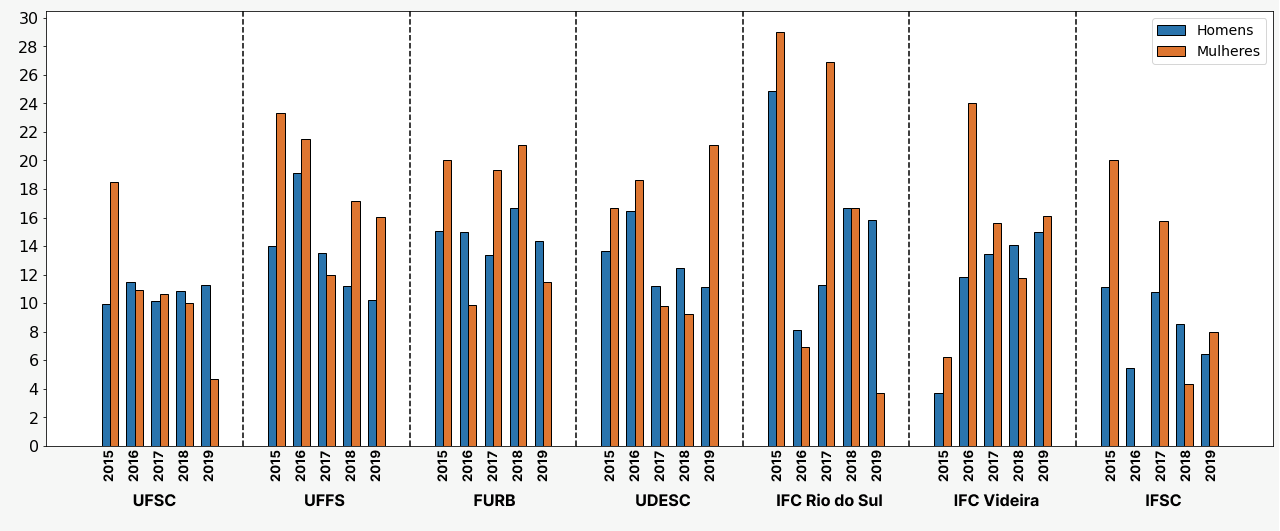
\includegraphics[width=0.93\textwidth]{taxa_de_evasao.png}
\caption{Taxas de Evasão Anuais por Instituição, Gênero e Ano}
\label{fig:exampleFig2}
\end{figure}

\subsection{Evasão por gênero e idade}\label{graf:generoeidade}
No conjunto de dados observado, a diferença de idade máxima encontrada entre homens e mulheres foi bastante significativa, sendo 61 anos para homens e 48 anos para mulheres. Essa faixa etária, porém, é pouco presente no curso, que possui estudantes com uma idade média de 22 anos, tanto para homens quanto para mulheres. Portanto, considerando os dados anteriores, o intervalo de análise mínimo proposto foi de até 25 anos, com intervalo máximo de mais de 55 anos. 

Estes dados compuseram o gráfico da Figura \ref{fig:exampleFig4}, que apresenta a relação entre gênero, idade e taxa de evasão nos anos observados. Um dos pontos críticos, onde houve maior evasão do gráfico ocorreu em 2016, em que, considerando apenas o número total de homens com idade entre 46 a 55 anos, 42,86\% daqueles que estavam nessa faixa etária evadiram. Para mulheres, o ponto de máxima percentual ocorreu nos anos de 2016 e 2019, na faixa etária de 26 a 35 anos, em que 28,57\% das mulheres contidas nessa faixa de idade evadiram. Além disso, percebe-se que as menores taxas de evasão são de estudantes com faixa etária de até 25 anos e que há uma tendência de crescimento desse número na medida em que se analisa estudantes mais velhos. É importante pontuar que quadrados que não possuem a porcentagem de evasão e aparecem sem cor estão dessa forma pois nos anos analisados não havia estudantes naquela faixa etária, e portanto não é possível concluir sobre a taxa de evasão para ela.

\begin{figure}[ht]
\centering
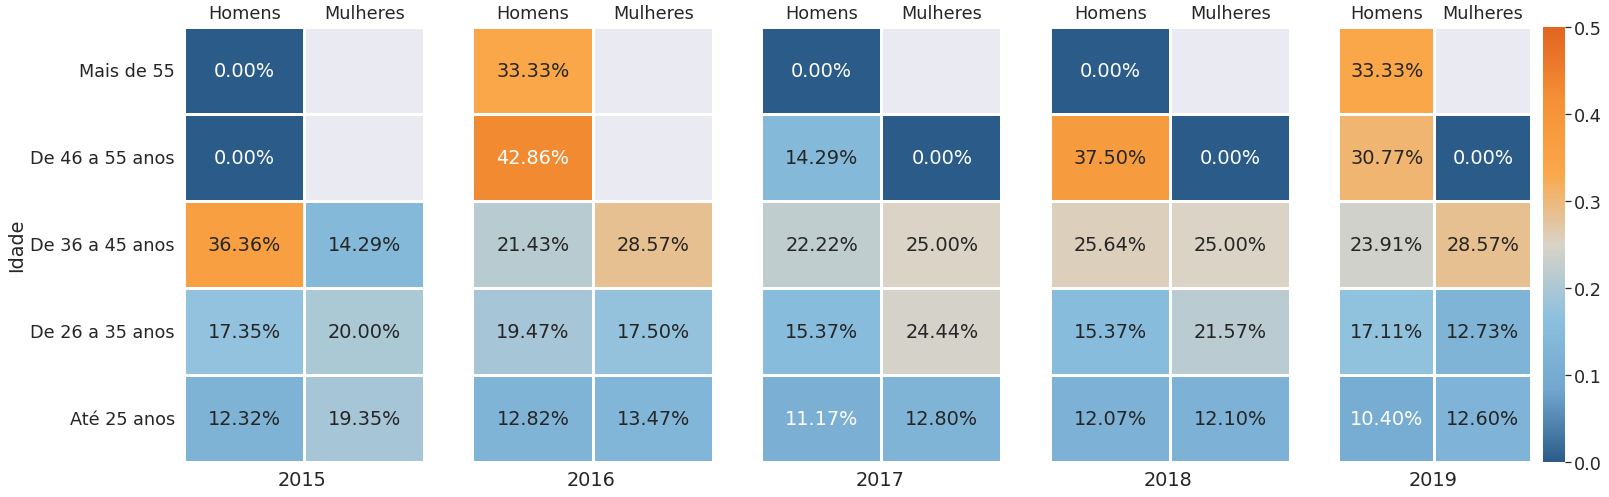
\includegraphics[width=1\textwidth]{Evasão por gênero e idade.png}
\caption{Taxa de Evasão Por Gênero e Idade no Ensino Superior}
\label{fig:exampleFig4}
\end{figure}





\subsection{Evasão por gênero e forma de ingresso}\label{graf:generoeformadeingresso}
Para a apresentação do gráfico da Figura \ref{fig:exampleFig5}, as categorias não nulas presentes na base de dados recortada são referentes à forma com que o estudante ingressou na Instituição de Ensino Superior.


\begin{figure}[ht]
\centering
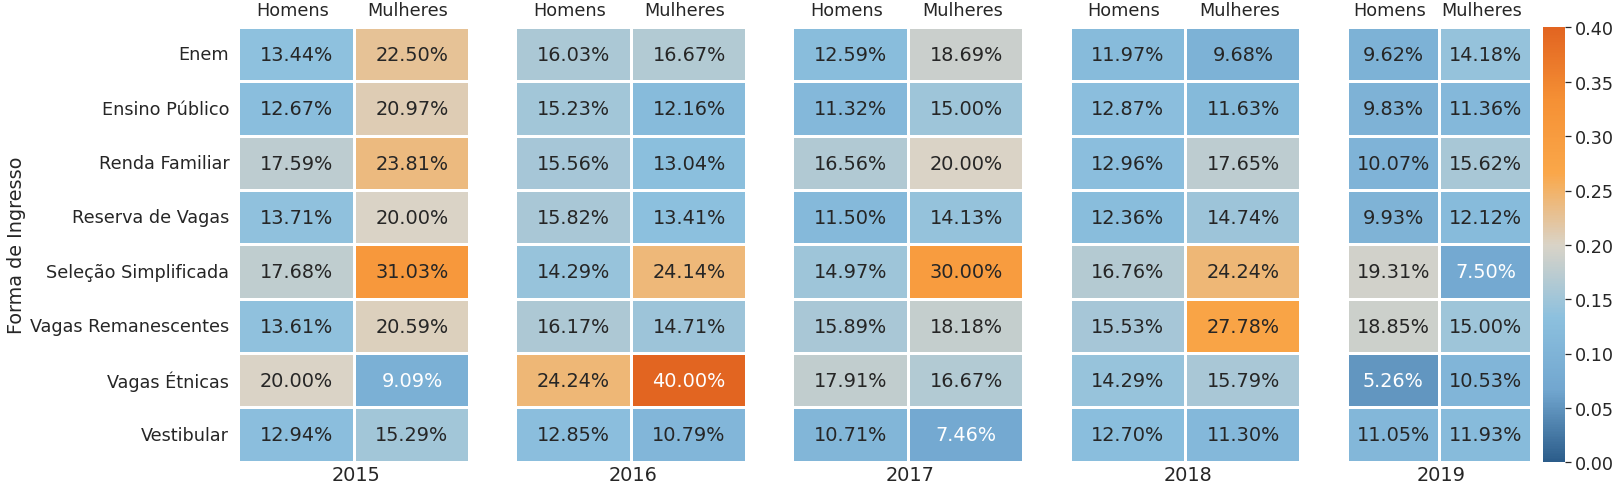
\includegraphics[width=1\textwidth]{Evasão por gênero e forma de ingresso.png}
\caption{Taxa de Evasão Por Gênero e Forma de Ingresso no Ensino Superior}
\label{fig:exampleFig5}
\end{figure}

A análise das formas de ingresso nas instituições citadas está presente na Figura \ref{fig:exampleFig5}, relacionando-se com gênero e taxa de evasão escolar por ano, desde 2015 até 2019. O ponto onde o gráfico possui a maior taxa de evasão pertence ao ano de 2016, onde, das mulheres que ingressaram pelo programa de vagas étnicas, 40\% evadiram. Percebe-se que há uma tendência bastante positiva de queda da taxa de evasão tanto feminina quanto masculina ao longo dos anos.





\subsection{Evasão por gênero e raça}\label{graf:generoeraca}

Nesta seção são apresentadas as informações quanto ao gênero, raça e taxa de evasão. Percebe-se na Figura \ref{fig:exampleFig6} que a evasão máxima em porcentagem ocorreu em 2016, onde 100\% das estudantes que se declaram como indígenas evadiram. Embora preocupante, esse valor é atrelado à baixa quantidade de mulheres pertencentes a essa etnia no curso, em que, nesse caso, a única mulher dessa categoria evadiu, levando a essa taxa tão elevada. 

Além disso, há vários pontos onde a taxa de evasão é zerada, significando que, dos estudantes evadidos daquele período, nenhum pertencia ao determinado grupo. Vale ressaltar que o recorte de mulheres autodeclaradas indígenas em 2015 está sem informações pois não haviam estudantes nesse grupo e período, portanto não é possível calcular sua taxa de evasão. 

\begin{figure}[ht]
\centering
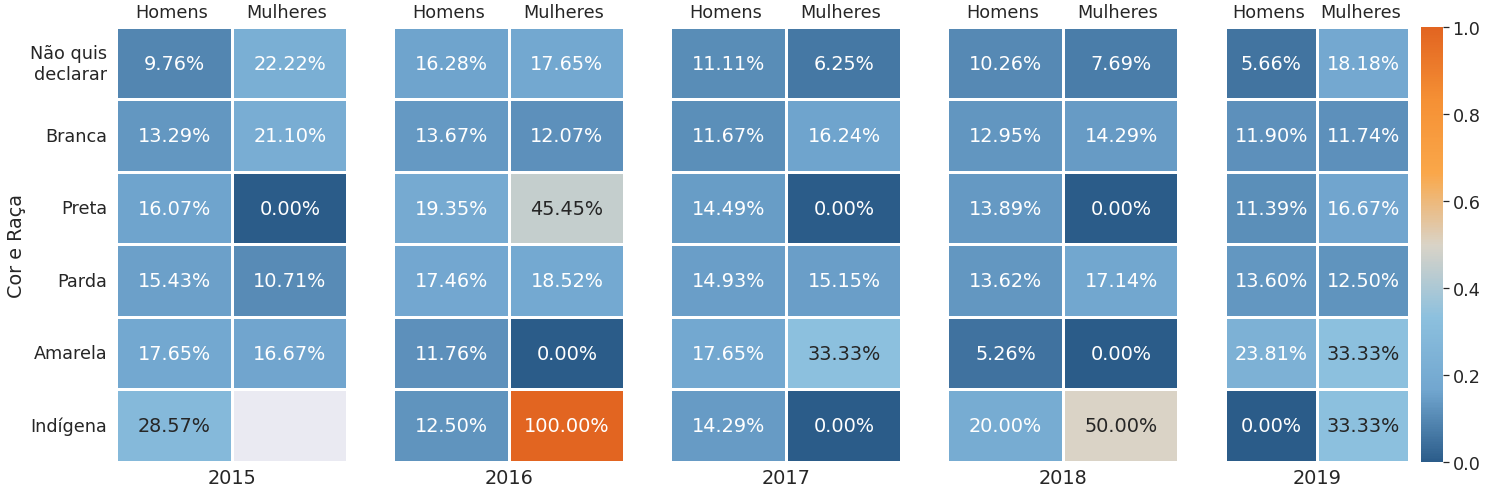
\includegraphics[width=1\textwidth]{Evasão por gênero e raca.png}
\caption{Taxa de Evasão Por Gênero, Cor e Raça no Ensino Superior}
\label{fig:exampleFig6}
\end{figure}




\section{Discussão dos Resultados}\label{discussaoresultados}

Partindo do que foi analisado ao longo do artigo, foi possível encontrar relações entre as variáveis abordadas. Com a observação dos gráficos das Figuras \ref{fig:MulheresHomens} e \ref{fig:exampleFig2}, juntamente com a Tabela \ref{tab:my-table} percebeu-se que os números absolutos de homens e mulheres nos cursos diferem muito, com um valor máximo de mulheres chegando a 67 em 2019 e um máximo de 519 homens em 2016. A maior diferença em porcentagem observada em uma mesma universidade ocorreu na UFSC em 2018, onde apenas 6,49\% dos estudantes do bacharelado de Ciência da Computação eram mulheres. Além disso, as taxas de evasão femininas ao longo dos anos tendem a ser superiores às masculinas, com a maior taxa de evasão feminina encontrada sendo de cerca de 29\%, enquanto a masculina máxima encontrada foi de pouco mais de 24\%, como é possível visualizar na Figura \ref{fig:exampleFig2}.

Outros pontos encontrados em decorrência da análise foram referentes ao intervalo etário dos estudantes, onde a idade máxima encontrada entre os homens matriculados foi de 61 anos, enquanto que nas mulheres essa máxima foi de apenas 48 anos na faixa de tempo observada. Ainda referente à idade, percebe-se que, à medida que aumenta a faixa etária, as taxas de evasão também aumentam para todos os estudantes. Além disso, para o intervalo de idade de até 25 anos, que compreende a idade média dos estudantes do curso, as taxas de evasão femininas foram maiores que as masculinas em todo o período observado.

A exploração das relações de raça e gênero na Figura \ref{fig:exampleFig6} mostraram que as taxas de evasão observadas entre os homens no ano de 2019, em sua maioria, foram as menores dos últimos 5 anos. Enquanto isso, esse fenômeno não pode ser observado para o gênero feminino, sendo visível apenas para as mulheres brancas. Assim, a redução da evasão feminina apontada anteriormente e pelos demais gráficos analisados não ocorre proporcionalmente entre todas as etnias. É importante pontuar que por conta do número reduzido de mulheres em certos grupos étnicos, a aparição de valores mais extremos de evasão, como zeros ou valores muito elevados, ocorrem com mais facilidade.   






\section{Considerações Finais}\label{consideracoesfinais}


Este artigo teve como principal objetivo a exploração sobre a evasão feminina nos cursos de Ciência da Computação. Para tal, foram definidas 5 questões de pesquisa. \textbf{Q1:} Qual a diferença entre estudantes homens e mulheres para cada instituição de ensino e ano analisados? \textbf{Q2:} Como se apresentam as taxas de evasão separadas por gênero nessas mesmas instituições e anos? \textbf{Q3:} Qual a relação entre faixa etária e gênero com a taxa de evasão? \textbf{Q4:} Qual a relação entre forma de ingresso no ensino superior e gênero com a taxa de evasão? \textbf{Q5:} Qual a relação entre raça e gênero com a taxa de evasão?

Todas as questões levantadas relacionam-se com as análises construídas no decorrer do artigo. A Questão 1 relaciona-se com as análises do capítulo \ref{sec:mulheresehomensgeral}, onde a diferença entre homens e mulheres mostra-se elevada. É possível notar tal diferença no gráfico da Figura \ref{fig:MulheresHomens} e também nos dados da Tabela \ref{tab:my-table}. Com isso, é possível observar a grande desigualdade de presença entre os gêneros nos cursos de Ciência da Computação das Instituições de Ensino Superior analisadas, chegando a ter 14 vezes mais homens do que mulheres.%ufsc 2018


A Questão 2 é respondida na Seção \ref{graf:generoanual}, em que nota-se que a evasão feminina tende a ser superior a masculina em todas as instituições de ensino superior, contudo, ao longo dos cinco anos explorados, há a redução da evasão tanto para homens quanto para mulheres. A Questão 3, que busca relacionar a faixa etária com gênero e taxa de evasão, foi respondida na Seção \ref{graf:generoeidade}, onde o mapa de calor apresentado demonstra que as taxas de evasão aumentam à medida que a faixa etária sobe, bem como discute sobre a disparidade de idades máximas encontradas entre matriculados homens e mulheres.

Já a Questão 4 analisa a relação entre as formas de ingresso e os gêneros com as taxas de evasão, sendo possível visualizar a resposta sobre essa relação analisando a Seção \ref{graf:generoeformadeingresso}, a qual apresenta a Figura \ref{fig:exampleFig5}, que mostra que a forma de ingresso onde ocorre as maiores taxas de evasão entre os gêneros, é na modalidade de vagas étnicas, chegando a apresentar taxas de evasão de 24,24\% e 40\% para homens e mulheres respectivamente no ano de 2016. Por fim, a Questão 5, que trata da análise entre raça e gênero, não conseguiu ser respondida com uma relação direta entre essas duas variáveis, ou seja, não há um padrão claro correspondente a todas as raças e seus gêneros, tendo os números apresentado bastante flutuação. As únicas exceções são a taxa de evasão de homens brancos, que mantêm-se constante de 11\% a 13\%, e a taxa de evasão dos homens pardos, que mantêm-se entre 13\% a 17\% em todos os cinco anos.

Como sugestões para trabalhos futuros, há a inclusão de mais estados nas análises além de Santa Catarina, para que se tenha uma visão mais ampla da situação brasileira da evasão escolar. Além disso, a inserção de outros cursos de \textit{STEM} permitiria ter um panorama melhor da área, possibilitando observar se os fenômenos que aparecem nas análises deste artigo se repetiram para outros cursos. Por fim, a adição de dados de universidades privadas permitiriam verificar se a situação observada é uma exclusividade do que foi analisado até o momento.

% \section{Figures, Tables and Captions}\label{sec:figs}

% O número de tabelas e figuras utilizadas no artigo deve ser limitado a compreensão e elucidação do texto. Devem ser inseridas no corpo do texto, para identificação da sua posição e do tamanho aproximado (Figura~\ref{fig:exampleFig1}).

% Tabelas e figuras possuem numeração independente, que deve ser feita seqüencialmente na ordem em que são citadas no texto. Devem também ter uma legenda auto-explicativa, sendo que as tabelas terão legendas na parte superior e as figuras as terão na parte inferior, centralizadas em relação à tabela ou figura. A legenda inicia com o termo "Tabela" ou "Figura" (primeira letra em maiúscula), de acordo com o caso, seguido de um espaço e do número de ordem seqüencial, em algarismos arábicos, seguido de hífen entre espaços e do texto da legenda, com a primeira letra da primeira palavra em maiúscula e as demais em minúscula, exceção feitas àquelas que normalmente são escritas em maiúsculas. Devem ser citadas no texto como "Tabela \ref{tab:exTable1}" e "Figura" seguidas de espaço e do número correspondente.

% \begin{figure}[ht]
% \centering
% 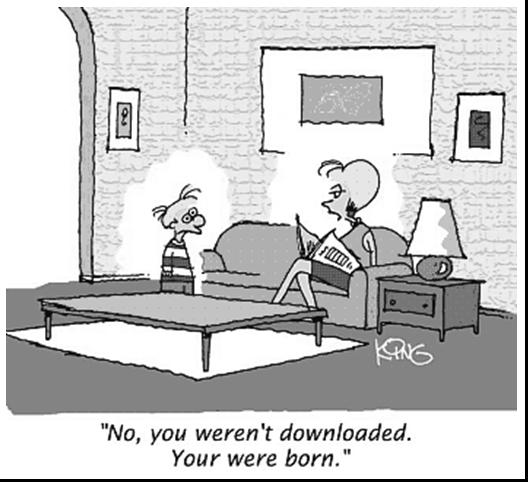
\includegraphics[width=.5\textwidth]{fig1.jpg}
% \caption{A typical figure}
% \label{fig:exampleFig1}
% \end{figure}

% \begin{figure}[ht]
% \centering
% 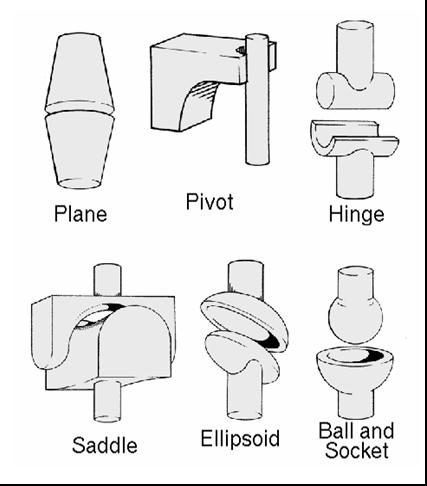
\includegraphics[width=.3\textwidth]{fig2.jpg}
% \caption{This figure is an example of a figure caption taking more than one
%   line and justified considering margins mentioned in Section~\ref{sec:figs}.}
% \label{fig:exampleFig2}
% \end{figure}

% \begin{table}[ht]
% \centering
% \caption{Variables to be considered on the evaluation of interaction
%   techniques}
% \label{tab:exTable1}
% 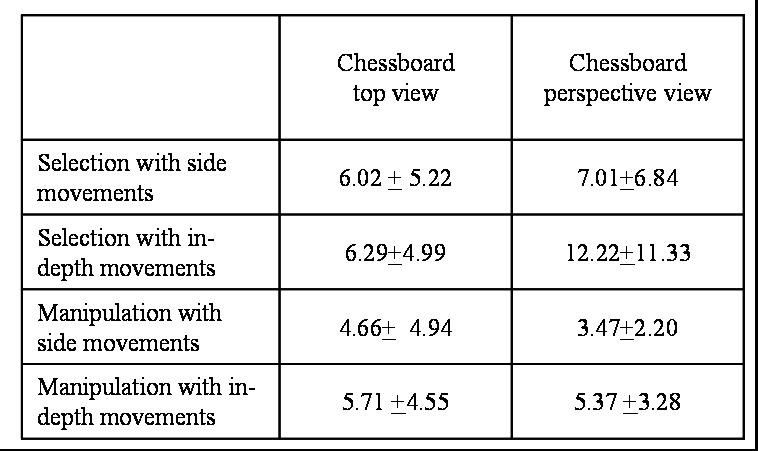
\includegraphics[width=.7\textwidth]{table.jpg}
% \end{table}

% \section{Referências}

% As referências a autores e fontes são inseridas no texto colocando entre parênteses o sobrenome do autor, com inicial maiúscula, seguida da data, conforme o exemplo: \cite{smith:99}. Quando for conhecida a paginação, pode-se incluí-la, por exemplo, (Tarouco, 1991, p. 237). Havendo mais de um título do(s) autor(es) no mesmo ano, deve-se distingui-las utilizando uma letra minúscula (a,b,c) depois da data, por exemplo, (Tarouco, 1991b). Quando houver três ou mais autores, no texto será citado apenas o primeiro autor seguido de "et al.", mas nas referências bibliográficas, no final do artigo, os demais nomes também deverão aparecer. Quando o nome do autor é citado diretamente no texto pode-se colocar entre parênteses apenas a data de publicação, por exemplo,

% \citeonline{boulic:91}. Na citação de citação, identifica-se a obra diretamente consultada; o autor e/ou a obra citada nesta é assim indicado: \cite{knuth:84} citada por Vicari \cite{teste}.

% As referências completas de cada autor e fonte citadas no texto devem aparecer no final do artigo sob o título "Referências Bibliográficas", ordenadas alfabeticamente pelo(s) sobrenomes(s) do(s) autore(s).

% Os autores do artigo devem certificar-se de que as referências citadas no texto contam da lista de referências com datas exatas e nomes de autores corretamente grafados. A exatidão dessas referências é de responsabilidade dos autores do artigo. Comunicações pessoais, trabalhos inéditos ou em andamento poderão ser citados quando absolutamente necessários, mas não devem ser incluídos na lista de referências bibliográficas; apenas citados no texto ou nas Notas do texto.

\addto{\captionsbrazil}{% caso use \usepackage[brazil]{babel}
\renewcommand{\bibname}{Refer\^{e}ncias Teses}
}
\bibliographystyle{renote}
\bibliography{References/references}

\end{document}
